% !TEX program = xelatex
\documentclass[UTF8,fontset=windows,12pt,a4paper]{ctexart}
\usepackage[a4paper,top=2.5cm,bottom=2.5cm,left=2.5cm,right=2.5cm]{geometry}
\usepackage{amsmath,amssymb,bm}
\usepackage{graphicx}
\usepackage{booktabs,longtable,array}
\usepackage{caption}
\usepackage{float}
\usepackage{setspace}
\usepackage{titlesec}
\usepackage{fancyhdr}
\usepackage{hyperref}
\hypersetup{hidelinks}
\setmainfont{Times New Roman}
\setCJKmainfont{SimSun}
\setCJKsansfont{SimHei}
\setCJKmonofont{FangSong}
\linespread{1.43}
\setlength{\parindent}{2em}
\setlength{\parskip}{0pt}
\pagestyle{fancy}
\fancyhf{}
\cfoot{\thepage}
\renewcommand{\headrulewidth}{0pt}
\titleformat{\section}{\centering\heiti\bfseries\zihao{3}}{}{0pt}{}
\titleformat{\subsection}{\heiti\bfseries\zihao{4}}{}{0pt}{}
\titleformat{\subsubsection}{\heiti\bfseries\zihao{-4}}{}{0pt}{}
\titlespacing{\section}{0pt}{1.0em}{0.6em}
\titlespacing{\subsection}{0pt}{0.8em}{0.35em}
\titlespacing{\subsubsection}{0pt}{0.6em}{0.25em}
\captionsetup{font=small,labelsep=quad}
\renewcommand{\arraystretch}{1.25}

\begin{document}
\begin{center}
{\heiti\bfseries\zihao{3} 基于多算法融合的无人机送货路径与能量优化模型}
\end{center}
\vspace{0.5em}

\begin{abstract}
本文研究城市短途小件配送中的无人机路径规划与能耗优化问题。针对单架无人机最短巡回、多架无人机协同配送以及复杂环境下燃料消耗最小化问题，分别建立旅行商模型、容量约束车辆路径模型和能耗约束自动化分配模型。

针对问题一，将单架无人机从仓库出发、遍历所有目的地并返回仓库的过程转化为旅行商问题，以总航程最短为目标建立闭合路径规划模型。当送货点数量  时采用全排列枚举法求全局最优解；当  时，先用最近邻法构造初始路径，再用 2-opt 算法优化。最终得到单架无人机最优路径为18-21-23-16-17-20-22-19-24-34-31-32-36-35-33-30-29-28-27-26-25-12-13-15-10-3-2-4-1-8-9-6-5-7-11-14-18，最短航程为2160.4529。

针对问题二，建立每架无人机最多访问 7 个目的地的容量约束车辆路径模型。首先计算各送货点相对于仓库的平面极角，采用扫描法完成初始分组；然后对各组内部全排列求最短路径，并通过组间两点交换降低总航程；最后枚举不同起始扫描角，选取最优方案。同时将天气、风速、时间、航程和燃料等因素作为路径可行性约束。计算得到多机最优分组方案为14-16-17-20-22-19-24，最短总航程为\raisebox{-0.25em}{\includegraphics[height=1.35em]{assets/asset_001.wmf}}。

针对问题三，考虑包裹载重、高度差、天气、风速及起降过程对燃料消耗和配送时间的影响，建立总燃料消耗最小的自动化分配模型。首先构造航段综合能耗函数；然后按包裹重量降序排序，采用最小能耗增量插入法生成初始方案；再通过路线内部调序、跨无人机包裹移位和两机包裹交换等启发式算子迭代优化。最终得到各无人机配送路线、初始装载重量、航段能耗和系统最低总能耗，最低总能耗为327.05。

本文模型由单机路径优化逐步扩展到多机协同和复杂环境能耗优化，结构清晰、算法可实现、结果便于解释。模型不足在于部分天气和能耗参数依赖假设，后续可结合实时气象数据和真实飞行数据进一步修正，并推广至动态订单、多仓库和异构无人机配送场景。
\end{abstract}
\noindent\textbf{关键词：}无人机配送 旅行商问题 车辆路径规划 扫描法 能耗优化
\section*{1. 问题的重述}
\addcontentsline{toc}{section}{1. 问题的重述}
\subsection*{1.1 问题一的重述}
在忽略天气、高度差和载重影响的条件下，安排一架无人机从仓库出发，遍历所有目的地后返回仓库，使总飞行距离最短。

\subsection*{1.2 问题二的重述}
在多架无人机共同配送时，每架无人机最多访问个目的地。需要将所有目的地合理分配给不同无人机，并为各无人机规划从仓库出发并返回仓库的配送航线，使所有无人机总航程最短；同时结合天气、风速、高度差、时间、燃料和航域等因素对路线进行约束与评价。

\subsection*{1.3 问题三的重述}
在多架无人机配送包裹且各无人机装载量相等的条件下，设计自动化分配方案，确定每架无人机负责的包裹及配送顺序，使系统总燃料消耗最少。本问题不考虑每架无人机的航程限制，但需考虑载重变化、天气、风速、高度差和起降过程对能耗的影响。

\section*{2. 问题的分析}
\addcontentsline{toc}{section}{2. 问题的分析}
\subsection*{2.1 问题一的分析}
问题一是单架无人机最短闭合路径问题。将仓库和目的地抽象为节点，将节点间距离作为边权，可转化为旅行商问题。点数较少时采用全排列法求精确最优解；点数较多时采用  最近邻法生成初始路径，再用t算法优化。

\subsection*{2.2 问题二的分析}
问题二属于带访问数量约束的多旅行商问题。本文先以仓库为极点计算各目的地的平面极角，利用扫描法将配送点划分为若干组，每组不超过 7 个点；再对组内路径全排列寻优，并通过组间两点交换和不同起始扫描角搜索降低总航程。天气、风速、高度差、时间、燃料和航域等因素作为路线可行性约束或辅助评价指标。

\subsection*{2.3 问题三的分析}
\subsection*{问题三的核心是装载量约束下的包裹分配与燃料消耗优化。无人机能耗与航段距离、当前载重、天气、风速、高度差及起降过程有关，且载重会随包裹送达逐渐下降。因此，本文建立考虑载重动态变化的能耗约束路径模型，采用最小能耗增量插入法生成初始方案，并通过路线内部调序、跨无人机移位和两机包裹交换进行迭代优化}
\subsection*{问题一模型的建立与求解}
\subsection*{5.1 一架无人机从起点出发历遍所有目的地返回出发点的最短路径}
\subsubsection*{5.1.1数据预处理：}
为获得后续建模所需的节点坐标信息，本文首先对原始地图进行预处理。具体而言，基于 HSV 颜色空间对图中不同颜色节点进行分割，并结合形态学运算去除噪声、修复区域。之后通过连通域分析提取节点质心坐标，对粘连节点采用聚类方法进行分离，最终完成所有节点的定位与坐标转换。在此基础上，构建节点间欧氏距离矩阵。结果如points.json所示。预处理结果表明，共识别有效节点 36 个，能够为后续模型建立提供可靠数据支撑。

\subsection*{5.2 最短路径模型：}
\subsubsection*{5.2.1模型解释：}
在完成节点识别与坐标提取后，需要确定一条从配送中心出发、遍历所有配送点并最终返回配送中心的最短闭合路径。该问题本质上属于经典的旅行商问题。旅行商问题的核心是在给定若干节点及其两两距离的条件下，寻找一条经过每个节点且仅经过一次、并回到起点的总路程最短路径。因此，本文将橙色节点视为配送中心，将绿色节点视为待配送点，建立单中心配送的旅行商优化模型。

\subsubsection*{5.2.2参数设定：}
设起点（仓库）为节点0所有点集合为\raisebox{-0.25em}{\includegraphics[height=1.35em]{assets/asset_002.wmf}}。两点\raisebox{-0.25em}{\includegraphics[height=1.35em]{assets/asset_003.wmf}}和\raisebox{-0.25em}{\includegraphics[height=1.35em]{assets/asset_004.wmf}}之间的直线距离为\raisebox{-0.25em}{\includegraphics[height=1.35em]{assets/asset_005.wmf}}。

\subsubsection*{5.2.3决策变量：}

\begin{center}\includegraphics[width=0.82\linewidth,height=0.23\textheight,keepaspectratio]{assets/asset_006.wmf}\end{center}

\subsubsection*{5.2.4目标函数：最小化总航程：}

\begin{center}\includegraphics[width=0.82\linewidth,height=0.23\textheight,keepaspectratio]{assets/asset_007.wmf}\end{center}

\subsubsection*{5.2.5约束条件：}
每个目的地必须且只能被访问一次（入度和出度均为1）：

每个节点只能离开一次：


\begin{center}\includegraphics[width=0.82\linewidth,height=0.23\textheight,keepaspectratio]{assets/asset_008.wmf}\end{center}

每个节点只能进入一次：


\begin{center}\includegraphics[width=0.82\linewidth,height=0.23\textheight,keepaspectratio]{assets/asset_009.wmf}\end{center}

\subsubsection*{5.2.6消除子回路约束（MTZ约束）：}
引入辅助变量\raisebox{-0.25em}{\includegraphics[height=1.35em]{assets/asset_010.wmf}}表示节点\raisebox{-0.25em}{\includegraphics[height=1.35em]{assets/asset_011.wmf}}在访问序列中的顺序：


\begin{center}\includegraphics[width=0.82\linewidth,height=0.23\textheight,keepaspectratio]{assets/asset_012.wmf}\end{center}

\subsubsection*{5.2.7变量取值约束：}

\begin{center}\includegraphics[width=0.82\linewidth,height=0.23\textheight,keepaspectratio]{assets/asset_013.wmf}\end{center}


\begin{center}\includegraphics[width=0.82\linewidth,height=0.23\textheight,keepaspectratio]{assets/asset_014.wmf}\end{center}

\subsubsection*{5.2.8综上}

\begin{center}\includegraphics[width=0.82\linewidth,height=0.23\textheight,keepaspectratio]{assets/asset_015.wmf}\end{center}


\begin{center}\includegraphics[width=0.82\linewidth,height=0.23\textheight,keepaspectratio]{assets/asset_016.wmf}\end{center}

\subsection*{问题一可归结为一个以总路径长度最小为目标的旅行商问题模型。该模型能够较好描述配送中心依次访问所有目标节点并返回起点的路径优化过程。}
\subsection*{5.3求解方法和结果}
\subsubsection*{5.3.1求解方法}
由于旅行商问题属于典型的组合优化问题，其求解复杂度随节点数增加迅速上升，因此本文根据节点规模采用分情况求解策略。当待配送节点数较少时，采用全排列枚举法求取精确最优解；当节点数较多时，采用最近邻算法生成初始路径，再结合 2-opt 局部优化算法进行改进，从而在保证求解效率的同时获得较优结果。


\begin{center}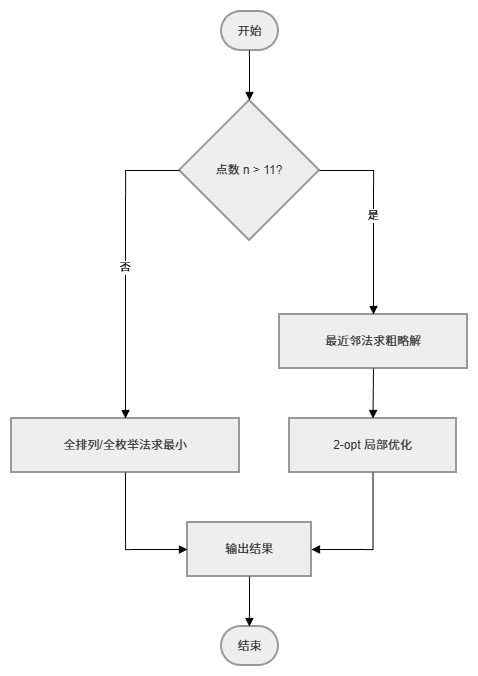
\includegraphics[width=0.82\linewidth,height=0.23\textheight,keepaspectratio]{assets/asset_017.png}\end{center}

\subsubsection*{5.3.2当  时的求解方法}
当待配送节点数较少时，所有可能路径的数量仍处于可接受范围内，因此本文采用全排列枚举法求解最优路径。具体做法是：固定蓝色配送中心为起点和终点，将其余n个配送节点的访问顺序进行全排列，构造所有可能的闭合路径，并逐一计算其总路径长度，最后选取总距离最短的路径作为最优解。

设一条可行路径表示为


\begin{center}\includegraphics[width=0.82\linewidth,height=0.23\textheight,keepaspectratio]{assets/asset_019.wmf}\end{center}

其中 \raisebox{-0.25em}{\includegraphics[height=1.35em]{assets/asset_020.wmf}} 为配送节点的一种排列，则该路径总长度为


\begin{center}\includegraphics[width=0.82\linewidth,height=0.23\textheight,keepaspectratio]{assets/asset_021.wmf}\end{center}

其中规定\raisebox{-0.25em}{\includegraphics[height=1.35em]{assets/asset_022.wmf}}\raisebox{-0.25em}{\includegraphics[height=1.35em]{assets/asset_023.wmf}}。

对所有可能的排列进行比较，可得全局最优解，即


\begin{center}\includegraphics[width=0.82\linewidth,height=0.23\textheight,keepaspectratio]{assets/asset_024.wmf}\end{center}

该方法属于精确求解方法，能够保证所得结果为全局最优解，但随着节点数增加，排列数呈阶乘增长，计算复杂度较高，因此只适用于小规模情形。

\subsubsection*{5.3.3当  时的求解方法}
当待配送节点数较多时，若仍采用全排列枚举法，计算量将迅速增大，难以在合理时间内完成求解。因此，本文采用“最近邻算法 + 2-opt 局部优化”的两阶段求解策略。第一阶段，利用最近邻算法构造初始路径。具体而言，从配送中心出发，在每一步都选择与当前节点距离最近的未访问节点作为下一访问节点，直至所有节点均被访问，最后返回配送中心，从而得到一条初始可行路径。第二阶段，在初始路径基础上采用 2-opt 局部优化算法。该方法通过交换路径中两条边的连接方式，对中间路径段进行反转，若交换后总路径长度减小，则接受该调整；重复执行该过程，直到路径无法继续改进为止。若原路径中两条边分别为 \raisebox{-0.25em}{\includegraphics[height=1.35em]{assets/asset_026.wmf}} 和 \raisebox{-0.25em}{\includegraphics[height=1.35em]{assets/asset_027.wmf}}，则 2-opt 交换后变为\raisebox{-0.25em}{\includegraphics[height=1.35em]{assets/asset_028.wmf}}和 \raisebox{-0.25em}{\includegraphics[height=1.35em]{assets/asset_029.wmf}}。当满足\raisebox{-0.25em}{\includegraphics[height=1.35em]{assets/asset_030.wmf}}时，说明交换后路径更优，可用新的连接方式替代原有连接方式。该方法不能保证得到全局最优解，但计算效率较高，且能够在较短时间内获得质量较好的近似最优解，适用于中大规模旅行商问题

\subsubsection*{5.3.4结果}
我们在忽略天气、载重和高度差等因素的条件下，将单架无人机配送路径优化问题抽象为旅行商问题。以仓库为起点和终点、各收货地点为中间访问节点，建立以总航程最短为目标的优化模型，并采用 2-opt方法 进行求解。计算结果表明，如表所示

\subsection*{问题一求解结果}
\begin{center}\small
\begin{longtable}{p{0.22\linewidth}p{0.22\linewidth}p{0.22\linewidth}p{0.22\linewidth}}
\toprule
点数 & 访问序列 & 总航程 &  \\
\midrule
35 & 18-21-23-16-17-20-22-19-24-34-31-32-36-35-33-30-29-28-27-26-25-12-13-15-10-3-2-4-1-8-9-6-5-7-11-14-18 & 2160.45 &  \\
\bottomrule
\end{longtable}
\end{center}
最优路径为：

18→21→23→16→17→20→22→19→24→34→31→32→36→35→33→30→29→28→27→26→25→12→13→15→10→3→2→4→1→8→9→6→5→7→11→14→18

最短距离


\begin{center}\includegraphics[width=0.82\linewidth,height=0.23\textheight,keepaspectratio]{assets/asset_031.wmf}\end{center}

\subsection*{5.4模型评价}
本文将无人机从仓库出发、依次访问所有配送点并最终返回仓库的配送过程抽象为旅行商问题，以无人机完成一次闭合配送任务的总航程最小为优化目标。根据各配送点的位置计算节点间距离，并采用最近邻算法生成初始路径，在此基础上利用 2-opt 算法不断交换路径中的边，以消除不合理的交叉路径并进一步缩短总航程。最终得到一条覆盖全部 35 个配送点且返回仓库 18 的可行路径，其总航程为 2160.4529。该模型能够较好地描述单架无人机、单一仓库条件下的配送路径规划问题。模型的目标函数明确，路径连续性、配送点唯一访问以及返回仓库等约束能够保证所得路径满足基本配送要求。最近邻算法计算速度较快，能够在较短时间内生成可行初始解；2-opt 算法则能够有效改善初始路径，减少路径交叉和不必要的绕行。两种算法结合后，在保证计算效率的同时，可以获得质量较高的配送方案，适合处理本题包含较多配送点的路径规划问题。但该模型仍存在一定局限性。首先，最近邻算法和 2-opt 算法均属于启发式算法，容易受到初始路径和局部搜索范围的影响，因此目前得到的路径只能称为当前算法搜索到的较优可行路径，不能严格证明其为全局最优路径。后续可以从三个方面对模型进行改进。一是采用多起点最近邻算法，分别以不同配送点生成初始访问顺序，再使用 2-opt 或 3-opt 算法进行局部优化，以降低初始路径对最终结果的影响；二是引入遗传算法、模拟退火算法或蚁群算法等全局搜索方法，提高跳出局部最优解的能力；三是将无人机载重、续航能力、配送时间窗、风场和禁飞区域等因素加入约束条件，建立更加符合实际配送需求的车辆路径模型。对于规模较小的问题，还可以使用整数规划、分支定界法等精确算法计算最优解或理论下界，从而评价启发式算法所得路径的优化程度。

\subsection*{5.2 问题二模型的建立与求解}
\subsubsection*{5.2.1 模型准备}
问题二要求在多架无人机共同配送的情况下，安排各无人机的配送航线，使总航程最短，并满足每架无人机最多访问个目的地的约束。根据题意，将仓库记为节点，将个  配送目的地记为节点 。各节点的平面坐标为，高度为。

首先，根据各配送点与仓库之间的相对位置，计算目的地相对于仓库的平面极角：


\begin{center}\includegraphics[width=0.82\linewidth,height=0.23\textheight,keepaspectratio]{assets/asset_032.wmf}\end{center}

为避免象限判断误差，实际计算中采用\raisebox{-0.25em}{\includegraphics[height=1.35em]{assets/asset_033.wmf}}函数：


\begin{center}\includegraphics[width=0.82\linewidth,height=0.23\textheight,keepaspectratio]{assets/asset_034.wmf}\end{center}

任意两个节点\raisebox{-0.25em}{\includegraphics[height=1.35em]{assets/asset_035.wmf}}之间的平面距离为：


\begin{center}\includegraphics[width=0.82\linewidth,height=0.23\textheight,keepaspectratio]{assets/asset_036.wmf}\end{center}

考虑城市不同地点高度差、天气和风速等因素对航线代价的影响，引入修正航程。设天气影响系数为\raisebox{-0.25em}{\includegraphics[height=1.35em]{assets/asset_037.wmf}}，风力影响系数为\raisebox{-0.25em}{\includegraphics[height=1.35em]{assets/asset_038.wmf}}，其中\raisebox{-0.25em}{\includegraphics[height=1.35em]{assets/asset_039.wmf}}与航段方向和风向有关。令\raisebox{-0.25em}{\includegraphics[height=1.35em]{assets/asset_040.wmf}}表示天气影响强度，\raisebox{-0.25em}{\includegraphics[height=1.35em]{assets/asset_041.wmf}}表示风力影响强度，则航段\raisebox{-0.25em}{\includegraphics[height=1.35em]{assets/asset_042.wmf}}的修正距离定义为：


\begin{center}\includegraphics[width=0.82\linewidth,height=0.23\textheight,keepaspectratio]{assets/asset_043.wmf}\end{center}

其中，当\raisebox{-0.25em}{\includegraphics[height=1.35em]{assets/asset_044.wmf}}时，模型退化为只考虑几何距离的普通路径规划模型；当\raisebox{-0.25em}{\includegraphics[height=1.35em]{assets/asset_045.wmf}}增大时，天气和风力因素对航线选择的影响增强。

约束条件：

每个目的地必须且只被服务一次


\begin{center}\includegraphics[width=0.82\linewidth,height=0.23\textheight,keepaspectratio]{assets/asset_046.wmf}\end{center}

每架无人机若执行任务，则从仓库出发一次


\begin{center}\includegraphics[width=0.82\linewidth,height=0.23\textheight,keepaspectratio]{assets/asset_047.wmf}\end{center}

每架无人机执行任务后必须返回仓库


\begin{center}\includegraphics[width=0.82\linewidth,height=0.23\textheight,keepaspectratio]{assets/asset_048.wmf}\end{center}


\begin{center}\includegraphics[width=0.82\linewidth,height=0.23\textheight,keepaspectratio]{assets/asset_049.wmf}\end{center}


\begin{center}\includegraphics[width=0.82\linewidth,height=0.23\textheight,keepaspectratio]{assets/asset_050.wmf}\end{center}

路径连续性约束


\begin{center}\includegraphics[width=0.82\linewidth,height=0.23\textheight,keepaspectratio]{assets/asset_051.wmf}\end{center}

每架无人机最多访问 7 个目的地


\begin{center}\includegraphics[width=0.82\linewidth,height=0.23\textheight,keepaspectratio]{assets/asset_052.wmf}\end{center}

禁止自环


\begin{center}\includegraphics[width=0.82\linewidth,height=0.23\textheight,keepaspectratio]{assets/asset_053.wmf}\end{center}

消除子回路约束


\begin{center}\includegraphics[width=0.82\linewidth,height=0.23\textheight,keepaspectratio]{assets/asset_054.wmf}\end{center}


\begin{center}\includegraphics[width=0.82\linewidth,height=0.23\textheight,keepaspectratio]{assets/asset_055.wmf}\end{center}

决策变量取值约束


\begin{center}\includegraphics[width=0.82\linewidth,height=0.23\textheight,keepaspectratio]{assets/asset_056.wmf}\end{center}

其中\raisebox{-0.25em}{\includegraphics[height=1.35em]{assets/asset_057.wmf}}为平面距离，\raisebox{-0.25em}{\includegraphics[height=1.35em]{assets/asset_058.wmf}}为比例尺，\raisebox{-0.25em}{\includegraphics[height=1.35em]{assets/asset_059.wmf}}为天气修正系数，\raisebox{-0.25em}{\includegraphics[height=1.35em]{assets/asset_060.wmf}}为风速修正系数


\begin{center}\includegraphics[width=0.82\linewidth,height=0.23\textheight,keepaspectratio]{assets/asset_061.wmf}\end{center}

没有考虑风速矢量和无人机飞行方向的夹角。它默认风只会增加燃料消耗，不区分顺风、逆风、侧风。优点是简单，缺点是物理意义较弱。\raisebox{-0.25em}{\includegraphics[height=1.35em]{assets/asset_062.wmf}}

其中\raisebox{-0.25em}{\includegraphics[height=1.35em]{assets/asset_063.wmf}}代表风速方向与航段\raisebox{-0.25em}{\includegraphics[height=1.35em]{assets/asset_064.wmf}}飞行方向的夹角，\raisebox{-0.25em}{\includegraphics[height=1.35em]{assets/asset_065.wmf}}代表城市平均风速，\raisebox{-0.25em}{\includegraphics[height=1.35em]{assets/asset_066.wmf}}代表无人机空速，\raisebox{-0.25em}{\includegraphics[height=1.35em]{assets/asset_067.wmf}}代表考虑风后的地速，\raisebox{-0.25em}{\includegraphics[height=1.35em]{assets/asset_068.wmf}}代表风速修正系数

\subsubsection*{5.2.2 多无人机路径规划模型}
设共有架无人机，每架无人机最多访问7个目的地。由于所有目的地都需要被配送，所需无人机数量至少为：


\begin{center}\includegraphics[width=0.82\linewidth,height=0.23\textheight,keepaspectratio]{assets/asset_069.wmf}\end{center}

设第\raisebox{-0.25em}{\includegraphics[height=1.35em]{assets/asset_070.wmf}}架无人机的配送路径为，则系统总修正航程为：


\begin{center}\includegraphics[width=0.82\linewidth,height=0.23\textheight,keepaspectratio]{assets/asset_071.wmf}\end{center}

问题二的目标函数为：


\begin{center}\includegraphics[width=0.82\linewidth,height=0.23\textheight,keepaspectratio]{assets/asset_072.wmf}\end{center}

约束条件如下。

每个目的地必须且只能被一架无人机访问：


\begin{center}\includegraphics[width=0.82\linewidth,height=0.23\textheight,keepaspectratio]{assets/asset_073.wmf}\end{center}

每架无人机最多访问 7 个目的地：


\begin{center}\includegraphics[width=0.82\linewidth,height=0.23\textheight,keepaspectratio]{assets/asset_074.wmf}\end{center}

每架无人机均从仓库出发并最终返回仓库：


\begin{center}\includegraphics[width=0.82\linewidth,height=0.23\textheight,keepaspectratio]{assets/asset_075.wmf}\end{center}

若某一航段受恶劣天气、强风或空域限制影响无法飞行，则将该航段设为不可行：


\begin{center}\includegraphics[width=0.82\linewidth,height=0.23\textheight,keepaspectratio]{assets/asset_076.wmf}\end{center}

其中，\raisebox{-0.25em}{\includegraphics[height=1.35em]{assets/asset_077.wmf}}表示目的地\raisebox{-0.25em}{\includegraphics[height=1.35em]{assets/asset_078.wmf}}由第\raisebox{-0.25em}{\includegraphics[height=1.35em]{assets/asset_079.wmf}}架无人机配送，否则为\raisebox{-0.25em}{\includegraphics[height=1.35em]{assets/asset_080.wmf}}；\raisebox{-0.25em}{\includegraphics[height=1.35em]{assets/asset_081.wmf}}表示第\raisebox{-0.25em}{\includegraphics[height=1.35em]{assets/asset_082.wmf}}架无人机从节点\raisebox{-0.25em}{\includegraphics[height=1.35em]{assets/asset_083.wmf}}飞往节点\raisebox{-0.25em}{\includegraphics[height=1.35em]{assets/asset_084.wmf}}，否则为\raisebox{-0.25em}{\includegraphics[height=1.35em]{assets/asset_085.wmf}}。

\subsubsection*{5.2.3 求解算法}
该问题属于带访问数量约束的多旅行商问题。若直接对所有目的地进行全局枚举，计算量较大。本文采用“极角扫描分组 + 组内全排列寻优 + 组间交换优化 + 多起点搜索”的启发式算法进行求解。

具体步骤如下：


\begin{center}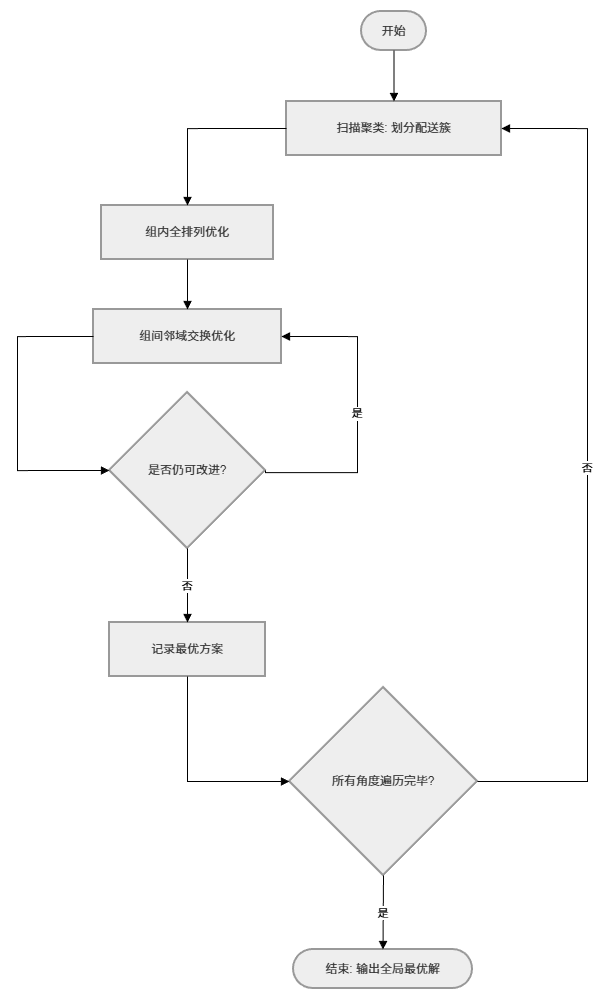
\includegraphics[width=0.82\linewidth,height=0.23\textheight,keepaspectratio]{assets/asset_086.png}\end{center}

Step 1：扫描聚类，划分配送簇。

首先计算所有配送点相对于仓库的平面极角\raisebox{-0.25em}{\includegraphics[height=1.35em]{assets/asset_087.wmf}}，并按照极角大小对配送点进行排序。然后从某一给定起始角度开始，沿顺时针方向扫描配送点，每次选取至多 7 个目的地作为一组，直到所有目的地均被划分到某一配送簇中。由此得到


\begin{center}\includegraphics[width=0.82\linewidth,height=0.23\textheight,keepaspectratio]{assets/asset_088.wmf}\end{center}

个配送组，每个配送组由一架无人机负责。

Step 2：组内全排列优化。

对每个配送组，枚举组内所有可能的目的地访问顺序。对于每一种访问顺序，利用航段修正航程函数\raisebox{-0.25em}{\includegraphics[height=1.35em]{assets/asset_089.wmf}}计算从仓库出发、依次访问组内目的地并返回仓库的闭合路径总修正航程。比较所有排列结果，选取修正航程最短的访问顺序作为该组当前最优路径。

Step 3：组间邻域交换优化。

任取两个配送组，记为第 p 组和第 q 组；再分别从两组中任取目的地 m 和 n，交换这两个目的地所属的配送组。交换后，重新对受影响的两个配送组进行组内全排列优化，并重新计算系统总修正航程。若交换后的总修正航程小于交换前，则接受该交换；否则拒绝该交换。

Step 4：判断是否仍可改进。

重复进行 Step 3 的组间邻域交换。若仍存在某一次交换能够降低系统总修正航程，则返回 Step 3 继续优化；若不存在任何能够降低总修正航程的交换，则认为当前起始角度下的分组与路径方案已经达到局部最优。

Step 5：记录当前最优方案。

当当前起始角度下无法继续改进时，记录该起始角对应的局部最优配送方案，包括各无人机负责的目的地集合、组内访问顺序以及系统总修正航程。

Step 6：判断所有角度是否遍历完毕。

改变扫描起始角度，重复 Step 1 至 Step 5，得到不同起始角度下的局部最优方案。若仍存在未遍历的起始角度，则返回 Step 1 重新进行扫描聚类；若所有起始角度均已遍历完毕，则进入最终比较。

Step 7：输出全局最优解。

比较所有起始角度下得到的局部最优方案，选取系统总修正航程最小的方案作为问题二的最终解，并输出各无人机的配送路径和对应修正航程。

\subsubsection*{5.2.4 求解结果}
取参数：


\begin{center}\includegraphics[width=0.82\linewidth,height=0.23\textheight,keepaspectratio]{assets/asset_090.wmf}\end{center}

经程序计算，共需无人机 5 架，系统总修正航程为：


\begin{center}\includegraphics[width=0.82\linewidth,height=0.23\textheight,keepaspectratio]{assets/asset_091.wmf}\end{center}


\begin{center}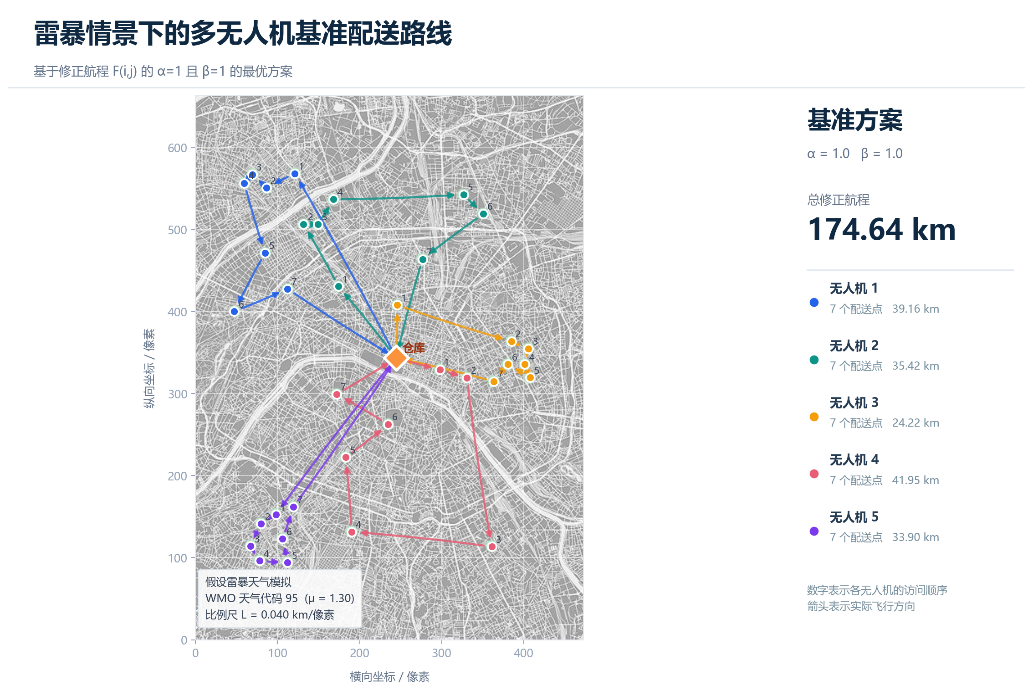
\includegraphics[width=0.82\linewidth,height=0.23\textheight,keepaspectratio]{assets/asset_092.png}\end{center}

各无人机配送路线如下表所示。

2-1 目的地访问顺序航线表

\begin{center}\small
\begin{longtable}{p{0.22\linewidth}p{0.22\linewidth}p{0.22\linewidth}}
\toprule
无人机 & 航线顺序 & 航程 /km \\
\midrule
1 & 1 → 4 → 2 → 3 → 10 → 15 → 13 & 39.160469 \\
2 & 12 → 8 → 9 → 6 → 5 → 7 → 11 & 35.416357 \\
3 & 14 → 16 → 17 → 20 → 22 → 19 → 24 & 24.217791 \\
4 & 21 → 23 → 34 → 31 → 27 → 26 → 25 & 41.947612 \\
5 & 29 → 30 → 33 → 35 → 36 → 32 → 28 & 33.896980 \\
\bottomrule
\end{longtable}
\end{center}
由结果可知，5 架无人机均满足每架最多访问 7 个目的地的约束。各组内部路线较为紧凑，说明基于极角扫描的初始分组能够较好地保持空间相邻性；组间交换进一步降低了总修正航程，提高了多机协同配送效率。

\subsubsection*{5.2.5 敏感性分析}

\begin{center}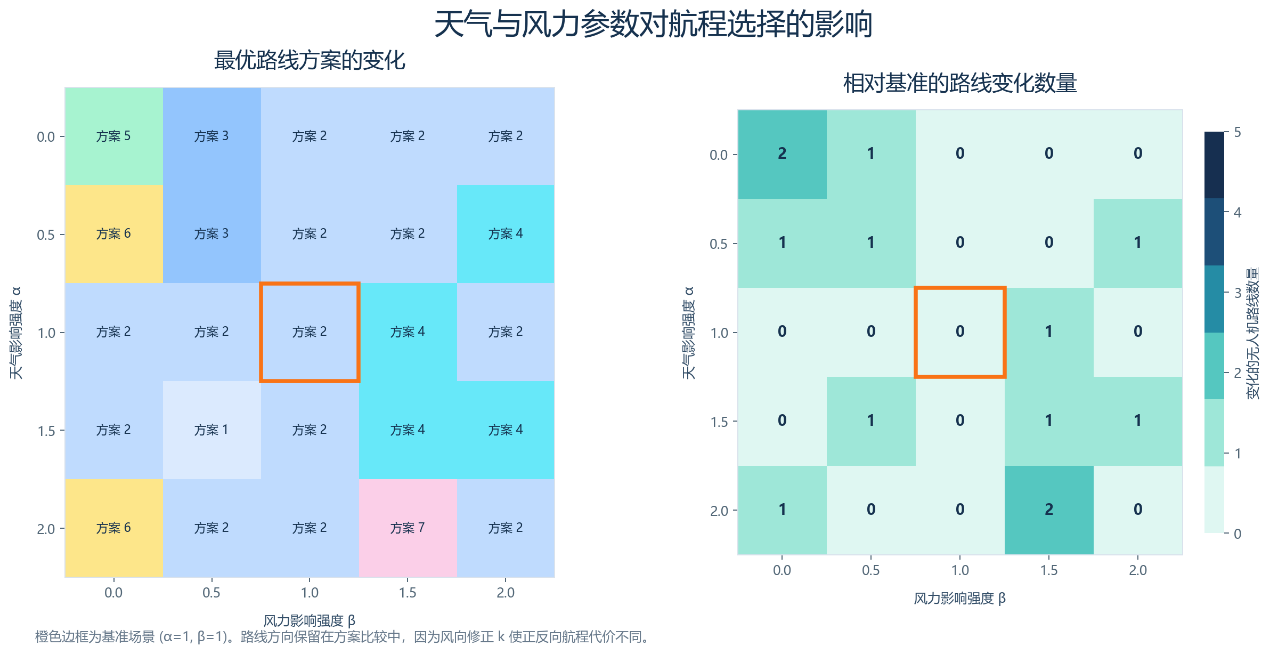
\includegraphics[width=0.82\linewidth,height=0.23\textheight,keepaspectratio]{assets/asset_093.png}\end{center}

为分析天气影响强和风力影响强度对模型结果的影响，以为基准场景，此时总修正航程为：


\begin{center}\includegraphics[width=0.82\linewidth,height=0.23\textheight,keepaspectratio]{assets/asset_094.wmf}\end{center}

\begin{center}{\small 表 1  固定 β=1 时 α 对总修正航程的影响}\end{center}
\begin{center}\small
\begin{longtable}{p{0.22\linewidth}p{0.22\linewidth}p{0.22\linewidth}}
\toprule
α & 总修正航程 /km & 相对基准变化 /\% \\
\midrule
0.0 & 134.338 & -23.08 \\
0.5 & 154.489 & -11.54 \\
1.0 & 174.639 & 0.00 \\
1.5 & 194.790 & +11.54 \\
2.0 & 214.941 & +23.08 \\
\bottomrule
\end{longtable}
\end{center}
\begin{center}{\small 表 2  固定 α=1 时 β 对总修正航程的影响}\end{center}
\begin{center}\small
\begin{longtable}{p{0.22\linewidth}p{0.22\linewidth}p{0.22\linewidth}}
\toprule
β & 总修正航程 /km & 相对基准变化 /\% \\
\midrule
0.0 & 169.788 & -2.78 \\
0.5 & 172.214 & -1.39 \\
1.0 & 174.639 & 0.00 \\
1.5 & 177.065 & +1.39 \\
2.0 & 179.491 & +2.78 \\
\bottomrule
\end{longtable}
\end{center}
由敏感性分析可知，在当前设定下，总修正航程对天气影响强度\raisebox{-0.25em}{\includegraphics[height=1.35em]{assets/asset_095.wmf}}更为敏感。当\raisebox{-0.25em}{\includegraphics[height=1.35em]{assets/asset_096.wmf}}由\raisebox{-0.25em}{\includegraphics[height=1.35em]{assets/asset_097.wmf}}增加到\raisebox{-0.25em}{\includegraphics[height=1.35em]{assets/asset_098.wmf}}时，总修正航程增加约 ；而当由增加到时，总修正航程仅增加约。因此，在本模型参数范围内，天气因素对总修正航程的影响明显大于风力因素。

进一步地，在 25 组参数组合中，总修正航程的最小值为，对应。；最大值为，对应。最大值相对基准增加约，最小值相对基准减少约。这说明模型结果会随环境影响强度变化而产生明显波动，验证了将天气和风力因素纳入修正航程模型的必要性。


\begin{center}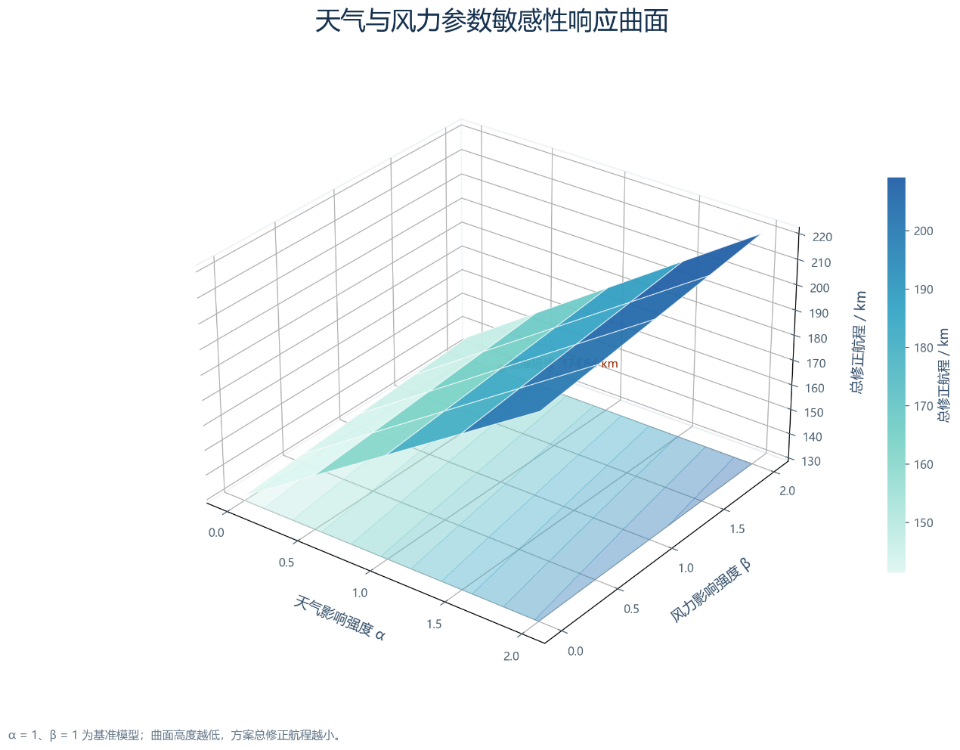
\includegraphics[width=0.82\linewidth,height=0.23\textheight,keepaspectratio]{assets/asset_099.png}\end{center}

\subsubsection*{5.2.6 结果评价}
本文建立的多无人机协同配送模型能够同时满足“每架无人机最多访问 7 个目的地”和“系统总航程最短”的要求。极角扫描法保证了初始分组的空间连续性，组内全排列法保证了单组路径的最优性，组间交换和多起始角搜索则进一步改善了全局方案。敏感性分析表明，模型对天气影响参数较为敏感，因此在实际应用中应优先获取较准确的天气数据，以提高航线规划结果的可靠性。

\subsection*{5.3 问题三的模型建立与求解}
\subsubsection*{5.3.1 问题三的模型建立}
A. 定义目标公式

在问题三中，由于我们仍然需要考虑关于天气和风向的约束，使得无人机在复杂状况下仍然能稳健地继续工作，并同时考虑无人机因需运送货物而产生额外载重，从而提高燃料的消耗速度，我们在问题二的基础上，定义无人机从  地飞到  地时的燃料成本目标函数如下。

\[G\left(i,j,t\right)=F\left(i,j\right)\times W(i,j,t)\]

其中， 是主体函数  的修正系数。由于无人机在途经不同收货点后会下放对应的包裹，从而减轻其载重，我们通过定义该修正系数来决定自无人机出发  时刻后，其实际载重对燃料消耗的影响因素。于是，我们考虑  将满足以下形式。

\[W\left(i,j,t\right)=1+η\times \frac{w\left(i,j,t\right)}{Q}\]

其中， 是  时刻下，对应无人机从  地飞往  地的当前载重； 是单个无人机的最大允许载重； 是相应的控制系数，它决定了无人机满载飞行时，其相对于空载飞行会增加多少比例的航段燃料消耗。另外，我们通过  进行了归一化处理，使得载重影响因素与相关物理单位无关，从而统一了量纲。

B. 单个无人机的燃料消耗函数

考虑对于某一架特定的无人机，其配送路线可考虑这样的表示。

\[{R}_{k}=\left({v}_{k,0},{v}_{k,1},…,{v}_{k,{m}_{k}},{v}_{k,{m}_{k+1}}\right)\]

其中，构成  的各个元素表示一个收获地点，并且  与  应是相同的点，因为起始点和返航点相同。 则指示无人机  在第  配送时应访问的收货点（或者说，在完成前  个收货点的任务后，应访问的下一个收货点）， 则指示该无人机所需要配送的任务总数（或者说，除开起点和终点外，所途经的收货点的数量）。

该无人机  按  依次完成路线上的包裹配送，并在完成全部任务后返回起点。记  指示该无人机在第  个配送点应卸载的包裹重量，则该无人机在抵达第  个配送点前的剩余载重可表示为如下形式。

\[{q}_{k,i}=\sum _{j=i}^{{m}_{k}} {d}_{k,j}\]

于是， 可考虑形式化为：

\[W\left(i,j,t\right)={W}_{i,j,k,r}=1+η\times \frac{{q}_{k,r}}{Q}\]

于是有：

\[G\left(i,j,t\right)={G}_{i,j,k,r}=F\left(i,j\right)\times {W}_{i,k,k,r}=F(i,j)\times \left(1+η\times \frac{{q}_{k,r}}{Q}\right)\]

同时考虑返航成本：

\[F\left({v}_{k,{m}_{k}},{v}_{k,{m}_{k+1}}\right)=F\left({v}_{k,{m}_{k}},0\right)\]

则单个无人机  的总燃料消耗评估函数为：

\[{E}_{k}=\left(\sum _{i=1}^{{m}_{k}} F\left({v}_{k,i-1},{v}_{k,i}\right)\left(1+η\times \frac{{q}_{k,i}}{Q}\right)\right)+F\left({v}_{k,{m}_{k}},0\right)\]

C. 多个无人机的总体评估函数

设  为某个方案所使用的无人机所组成的集合，则所有无人机的燃料消耗的评估总和为：

\[{E}_{total}=\sum _{k\in K}^{} {E}_{k}\]

考虑最小化燃料消耗，则应求解：

\[min{E}_{total}=min\sum _{k\in K}^{} {E}_{k}\]

即：

\[min{E}_{total}=min\sum \sum _{k\in K}^{} \left(\left(\sum _{i=1}^{{m}_{k}} F\left({v}_{k,i-1},{v}_{k,i}\right)\left(1+η\times \frac{{q}_{k,i}}{Q}\right)\right)+F\left({v}_{k,{m}_{k}},0\right)\right)\]

D. 约束条件

设全部包裹所组成的集合为 ，无人机  要运送的包裹为 ，其中 ，由于考虑到每个包裹只能被配送依次，则有：

\[⋃_{k\in K}^{} B{g}_{k}=Bg\]

且对于任意两个不同的无人机  和  有：

\[\left(B{g}_{k}⋂B{g}_{l}\right)=0\]

这意味着每个各个无人机获得的配送集合本质上构成了对总配送集合的划分。这意味着每个包裹既不能遗漏，也不能被重复分配到不同的无人机上。

另外，对于方案中的任意一个无人机  而言，应确保其最初驶离起点前，其初始载重不超过单个无人机的最大载重，即：

\[∀\left(k\in K\right),∃\left(\sum _{i=1}^{{m}_{k}} {d}_{k,i}\le Q\right)\]

最后应保证每个包裹的重量是正实数，即：

\[{d}_{k,i}>0,   ∀i\]

E. 总体模型

\[min{E}_{total}=min\sum \sum _{k\in K}^{} \left(\left(\sum _{i=1}^{{m}_{k}} F\left({v}_{k,i-1},{v}_{k,i}\right)\left(1+η\times \frac{{q}_{k,i}}{Q}\right)\right)+F\left({v}_{k,{m}_{k}},0\right)\right)\]

\[s.t.\left(\begin{aligned}{q}_{k,i}=\sum _{j=i}^{{m}_{k}} {d}_{k,j} \\ {v}_{k,0}={v}_{k,{m}_{k+1}} \\ F\left({v}_{k,{m}_{k}},{v}_{k,{m}_{k+1}}\right)=F\left({v}_{k,{m}_{k}},0\right) \\ ⋃_{k\in K}^{} B{g}_{k}=Bg \\ \left(B{g}_{k}⋂B{g}_{l}\right)=0,k\ne l \\ ∀\left(k\in K\right),∃\left(\sum _{i=1}^{{m}_{k}} {d}_{k,i}\le Q\right) \\ {d}_{k,i}>0, ∀i \\ F\left(i,j\right)=d\left(i,j\right)\times L\times \mu \times η\left({v}_{w},{v}_{a},i,j\right) \\ η\left({v}_{w},{v}_{a},i,j\right)=\frac{{v}_{a}}{{v}_{g,ij}} \\ {v}_{g,ij}=\sqrt{{v}_{a}^{2}-{v}_{w}^{2}{sin}^{2}{\theta }_{ij}}+{v}_{w}cos{\theta }_{ij} \\ \mu =\left(\begin{aligned}1,\&wc=0 \\ 1.01,\&1\le wc\le 3 \\ 1.08,\&wc\in \left(45,48\right) \\ 1.06,\&wc\in \left(51,53,55\right) \\ 1.18,\&wc\in \left(56,57,66,67\right) \\ 1.10,\&wc\in \left(61,63,65\right) \\ 1.15,\&wc\in \left(71,73,75,77\right) \\ 1.12,\&wc\in \left(80,81,82\right) \\ 1.18,\&wc\in \left(85,86\right) \\ 1.30,\&wc=95 \\ 1.50,\&wc\in \left(96,99\right)\end{aligned}\right)\end{aligned}\right)\]

\subsubsection*{5.3.2 问题三的模型求解}
A. 算法简述

Step 1. 构造初始近似解

Step 1.1. 将待配送的所有包裹按重量从大到小排序

Step 1.2. 对于待配送的每个包裹

Step 1.2.1. 将包裹插入已有路线

Step 1.2.2. 将包裹放入一架新的无人机

Step 1.2.3. 比较1.2.1和1.2.2的优劣性，并仅接受更优操作

Step 2. 对初始解进行多重邻近交换调优

Step 2.1. 对于每个无人机，在其内部的路线中交换途径点。如果找到更优解，则重新执行2.1

Step 2.2. 对于每个无人机，从其内部的途径点选取一点，并插入到其内部的所有可能位置。如果找到更优解，则重新执行2.1

Step 2.3. 选取两个无人机，从一个无人机中取出包裹，并放入另外一个无人机中，并尝试所有可能的途径点安排顺序。如果找到更优解，则重新执行2.1

Step 2.4. 选取两个无人机，并各从这两个无人机中选取一个包裹，然后交换，并尝试所有可能的途径点安排顺序。如果找到更优解，则重新执行2.1

Step 2.5. 此时仍然没有找到任何更优解，则跳转到第三步

Step 3. 输出目前的解作为答案，并终止程序

B. 程序逻辑框图


\begin{center}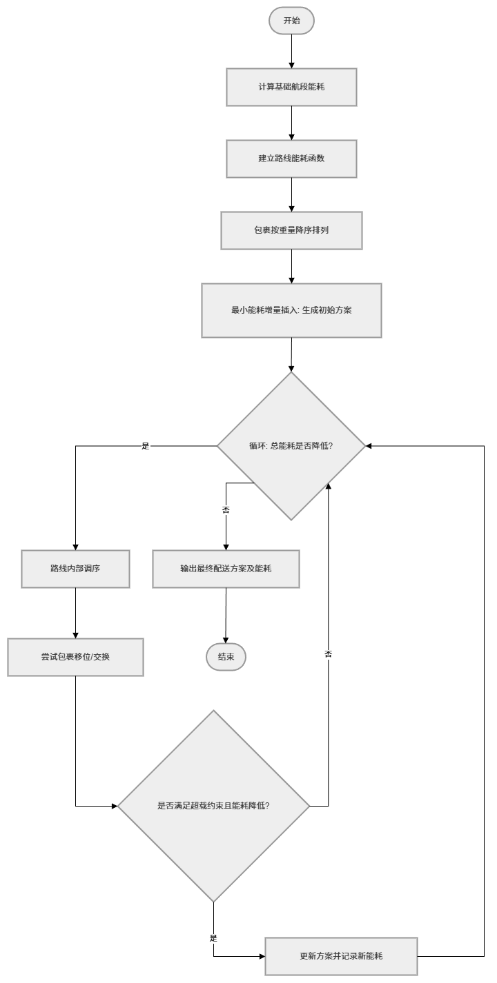
\includegraphics[width=0.82\linewidth,height=0.23\textheight,keepaspectratio]{assets/asset_100.png}\end{center}

\begin{center}{\small 图X 问题三算法求解程序框图}\end{center}
\subsubsection*{5.3.3 问题三模型求解结果}
\subsection*{问题三的求解继续沿用问题二的相关参数的基础上，并额外定义了一些常量。以下是求解问题时，本论文所定义的所有常量。}
\[\left(\begin{aligned}η=0.3 \\ L=0.004 \&km/pixel \\ {v}_{a}=50 \&km/s \\ wc=95 (⟹\mu =1.3)\end{aligned}\right)\]

为了求解该问题，本论文收集了巴黎当地的一些天气数据，并选取使用协调世界时2025/05/01 08:00的风速数据进行模型求解。

除此外，由于题目没有明确给出应派往各个收获点的包裹待派发列表，因此我们考虑自行生成一些包裹派发列表用于求解。对于生成派发列表的算法，它首先为每个配送点以68\%和32\%的概率分别生成1个或2个包裹，随后以50\%、35\%和15\%的概率将包裹划分为轻型、中型和重型，并分别在 、 和  kg 的区间内进行均匀抽样，同时固定随机种子以保证模拟实验可以在他处容易地复现。下面是生成的，并用作求解本问题的待派发列表数据。

\begin{center}{\small 表X 待配送的包裹待派发列表}\end{center}
\begin{center}\small
\begin{longtable}{p{0.22\linewidth}p{0.22\linewidth}p{0.22\linewidth}p{0.22\linewidth}}
\toprule
配送点 & 包裹重量 /kg & 包裹数 & 总重量 /kg \\
\midrule
1 & 1.13 & 1 & 1.13 \\
2 & 2.15 & 1 & 2.15 \\
3 & 2.66 & 1 & 2.66 \\
4 & 1.57 & 1 & 1.57 \\
5 & 1.50 & 1 & 1.50 \\
6 & 1.13, 2.34 & 2 & 3.47 \\
7 & 2.76 & 1 & 2.76 \\
8 & 3.96 & 1 & 3.96 \\
9 & 0.62 & 1 & 0.62 \\
10 & 0.33 & 1 & 0.33 \\
11 & 2.78 & 1 & 2.78 \\
12 & 1.19, 0.93 & 2 & 2.12 \\
13 & 0.79, 1.10 & 2 & 1.89 \\
14 & 1.08, 0.53 & 2 & 1.61 \\
15 & 2.37, 0.90 & 2 & 3.27 \\
16 & 0.48, 0.79 & 2 & 1.27 \\
17 & 0.41 & 1 & 0.41 \\
19 & 2.27 & 1 & 2.27 \\
20 & 1.18 & 1 & 1.18 \\
21 & 1.94 & 1 & 1.94 \\
22 & 1.14 & 1 & 1.14 \\
23 & 1.20 & 1 & 1.20 \\
24 & 0.96 & 1 & 0.96 \\
25 & 2.13, 1.74 & 2 & 3.87 \\
26 & 0.87 & 1 & 0.87 \\
27 & 0.63, 0.49 & 2 & 11.12 \\
28 & 1.08, 1.84 & 1 & 2.92 \\
29 & 0.98 & 1 & 0.98 \\
30 & 2.12 & 1 & 2.12 \\
31 & 1.01 & 1 & 1.01 \\
\bottomrule
\end{longtable}
\end{center}
待配送的包裹待派发列表（续表）

\begin{center}\small
\begin{longtable}{p{0.22\linewidth}p{0.22\linewidth}p{0.22\linewidth}p{0.22\linewidth}}
\toprule
配送点 & 包裹重量 /kg & 包裹数 & 总重量 /kg \\
\midrule
32 & 1.63, 2.03 & 2 & 3.66 \\
33 & 2.26 & 1 & 2.26 \\
34 & 3.99 & 1 & 3.99 \\
35 & 2.59, 2.58 & 2 & 5.17 \\
36 & 1.11, 2.16 & 2 & 3.27 \\
\bottomrule
\end{longtable}
\end{center}
通过运行求解如何运送这些包裹，我们最终使用了八架无人机。每架无人机的途径点、运送的包裹、载重变化量、相应路径下的  以及相应路径下的燃料消耗已经在下面两个示意图中标出。


\begin{center}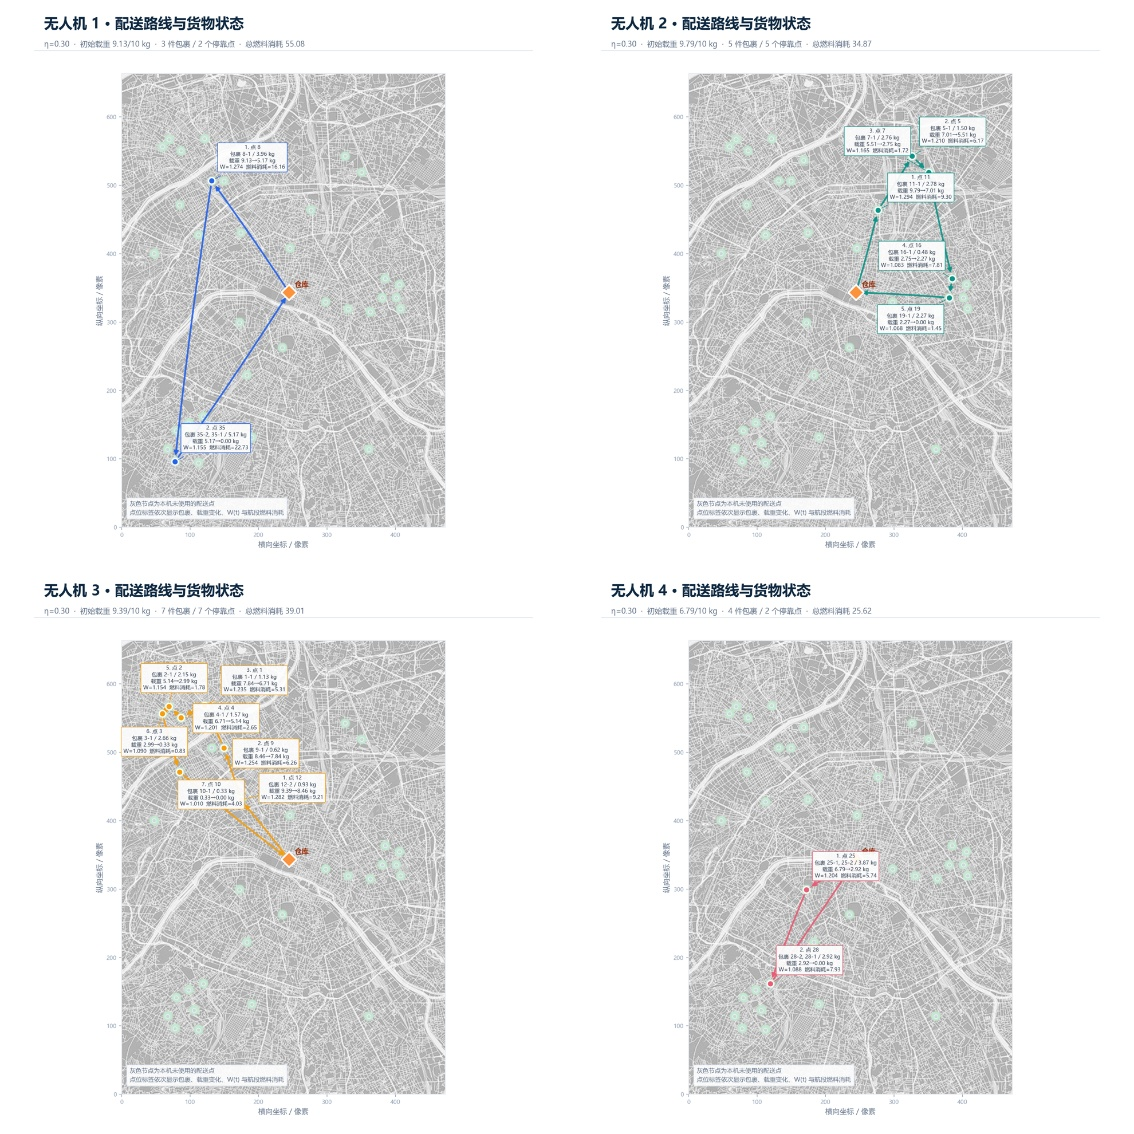
\includegraphics[width=0.82\linewidth,height=0.23\textheight,keepaspectratio]{assets/asset_101.jpeg}\end{center}

\begin{center}{\small 图X 问题三求解结果（一）}\end{center}

\begin{center}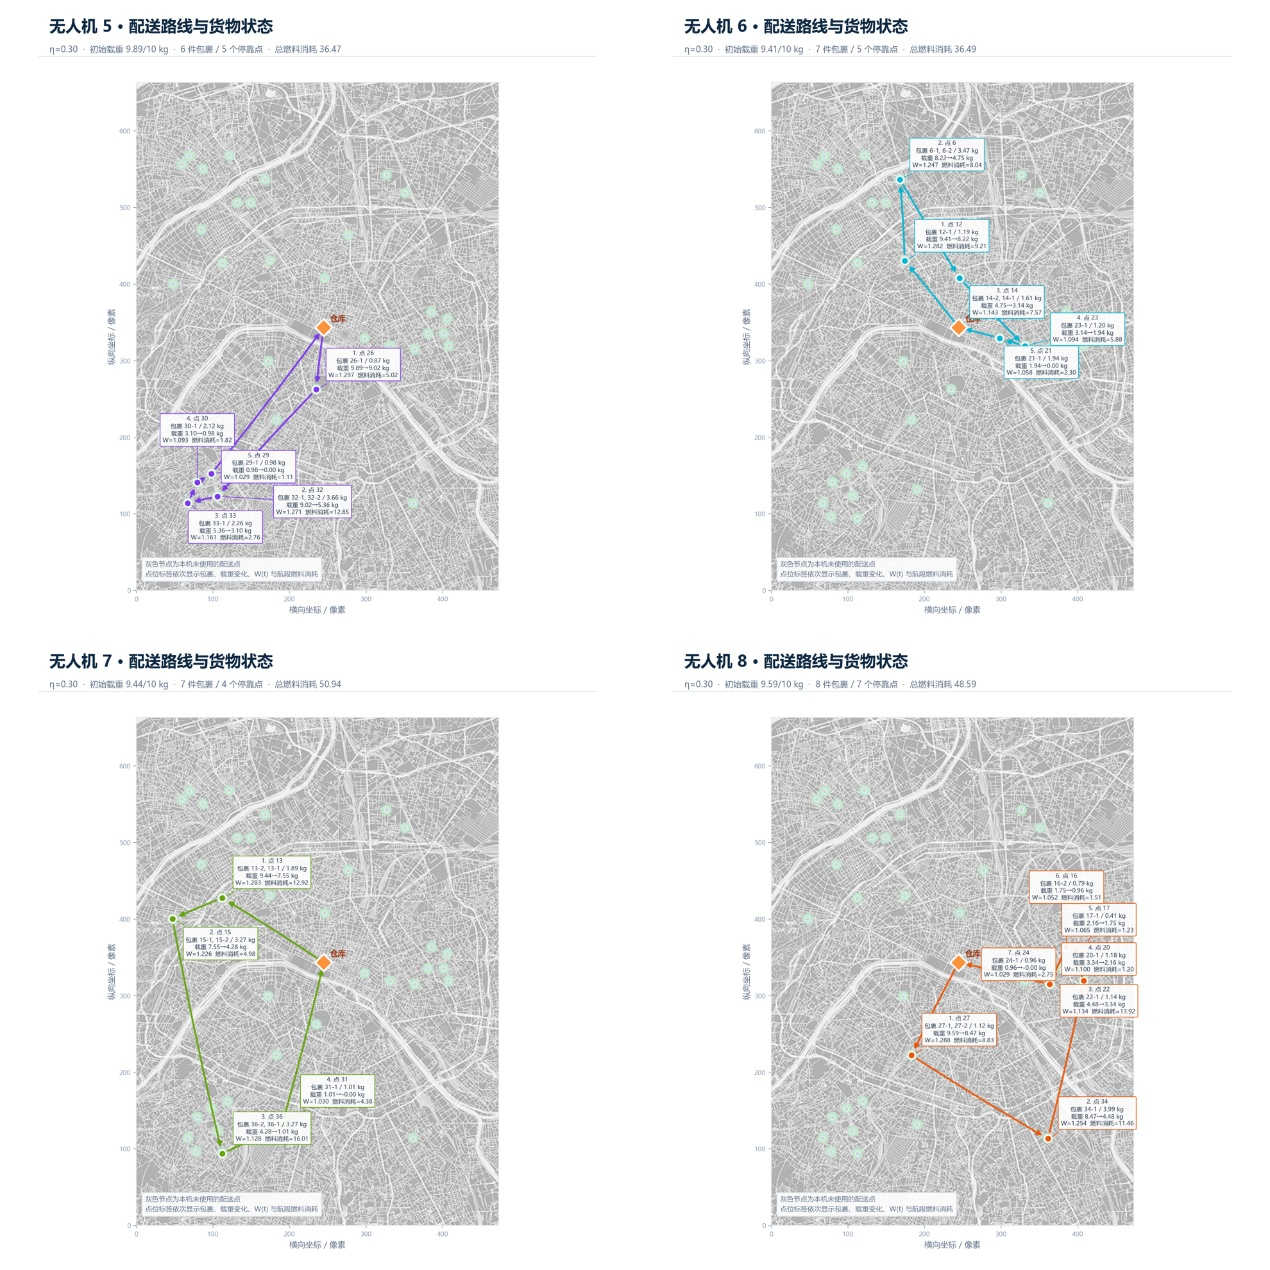
\includegraphics[width=0.82\linewidth,height=0.23\textheight,keepaspectratio]{assets/asset_102.jpeg}\end{center}

\begin{center}{\small 图X 问题三求解结果（二）}\end{center}
下图则综合地展示了所有无人机的运送路线，其中概述了各个无人机运送货物的基本信息，包括但不限于运送的货物总重量，以及模型求解出的最少燃料消耗。


\begin{center}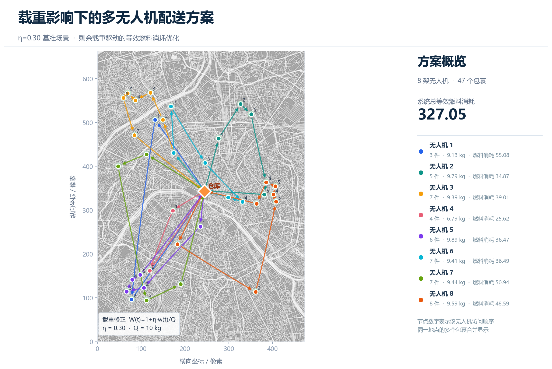
\includegraphics[width=0.82\linewidth,height=0.23\textheight,keepaspectratio]{assets/asset_103.png}\end{center}

\begin{center}{\small 图X 问题三综合求解结果}\end{center}
\subsubsection*{5.3.4 模型敏感性分析}
考虑  是未知参数，在5.3.3 其他常数设置不变的情况下，我们研究了下面所有  取值后的无人机包裹分配、路线规划结果。

\[η=0.01k,   k=1,2,3,…,n\]

这意味着  从0.01开始取值，每次步进0.01，一共步进99次，直到取到1，即一共取100个值。下图则展示了随  不断增大时，综合燃料消耗评估值  不断上升，包裹分配方案不断变化。


\begin{center}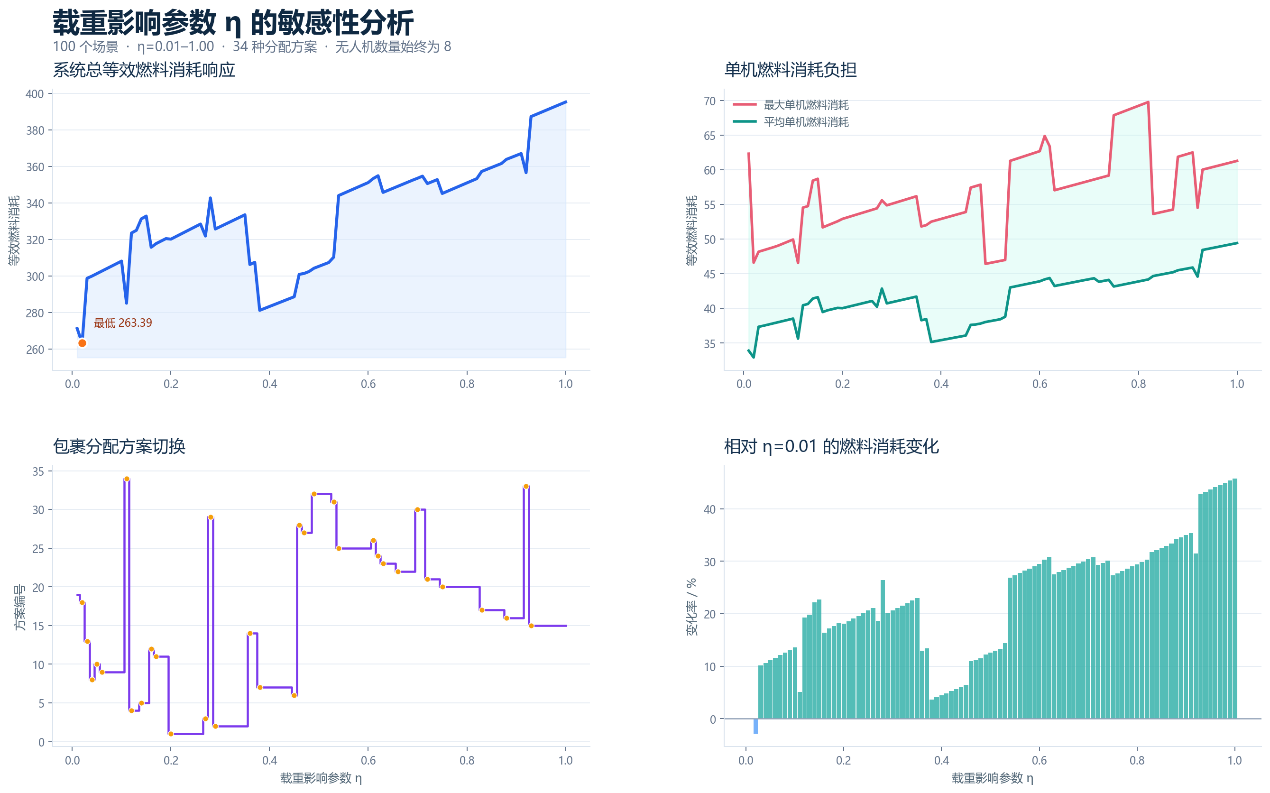
\includegraphics[width=0.82\linewidth,height=0.23\textheight,keepaspectratio]{assets/asset_104.png}\end{center}

\begin{center}{\small 图X 问题三/敏感性分析/可视化/示意图}\end{center}
这意味着  不只是对固定路线的燃料消耗做线性放大，还会影响该启发式算法选择的包裹分配和访问顺序。因为载重修正因子  与配送顺序有关，而重量更大的包裹可能更早被配送，后续行程的剩余载重下降越快，因而，算法会尝试将重包裹、长距离配送点和风力影响较大的地区和它对应的包裹进行更合理的规划和组合。然而，无论如何调整  的值，所有方案均采用8架无人机执行配送工作，这意味着它仅仅影响包裹的分配、每架无人机的途径各送货点的顺序，以及各个无人机的燃料消耗，但不构成对线路数量的显著影响。

当然，可以关注到总燃料消耗曲线总体上升，但可能存在局部下降。不过这可能不意味着增加载重影响后，燃料消耗会真正的下降，这可能是因为本模型的局限性。考虑到本模型考虑了多个参数，包括但不限于风力影响、天气影响，以及载重影响，采用暴力求解寻找最优解是不可能的，可能的解数目是不可计算的。然而，该模型通过使用近似法取得了局部最优解，但这并不保证是全局最优的，也意味着不同  参数下，对应的求解算法表现更好，会收敛到不同的局部最优路线，从而导致了观察到的下降趋势。

\subsubsection*{5.3.4 模型结论}
针对载重相关的多无人机配送路径规划问题，本文引入无量纲载重影响参数 ，并通过100组情景分析考察其影响。结果表明，随着  从0.01增加至1.00，系统等效燃料消耗总体由 271.207增加至395.324，增幅约为45.77\%，说明系统对载重效应具有较高敏感性。

取  作为基准情景时，系统使用8架无人机，等效燃料消耗为327.053。不同  情景共产生34种包裹分配方案，表明载重参数会影响无人机的任务分配和访问顺序。

然而，在当前包裹数据及10 kg单机最大载重约束下，无人机数量在各情景中均保持为8架。因此，载重影响参数主要改变燃料消耗水平和路线结构，而未改变当前实例所需的无人机数量。

\section*{参考文献}
\addcontentsline{toc}{section}{参考文献}
\begin{center}\small
\begin{longtable}{p{0.22\linewidth}p{0.22\linewidth}}
\toprule
[1] & VIDAL T. Hybrid genetic search for the CVRP: Open-source implementation and SWAP* neighborhood[J/OL]. Computers \& Operations Research, 2022, 140(105643): 105643-105643. DOI:10.1016/j.cor .2021.105643. \\
\midrule
[2] & ARIT THAMMANO, PETCHARAT RUNGWACHIRA. Hybrid modified ant system with sweep algorithm and path relinking for the capacitated vehicle routing problem[J/OL]. Heliyon , 2021, 7(9): e08029-e08029[2026-07-17]. DOI:10.1016/j.heliyon .2021.e08029. \\
[3] & ZHOU Y, LEE G. A Lagrangian Relaxation-Based Solution Method for a Green Vehicle Routing Problem to Minimize Greenhouse Gas Emissions[J/OL]. Sustainability, 2017, 9(5): 776[2026-07-17]. DOI:10.3390/su9050776. \\
[4] & RUZICKA M, BECVAR Z, GAZDA J. Energy Consumption Optimization for UAV Base Stations With Wind Compensation[J/OL]. IEEE Communications Letters, 2023, 27(4): 1210-1214[2026-07-17]. DOI:10.1109/lcomm.2023.3249630. \\
[5] & ZENG Y, XU J, ZHANG R. Energy Minimization for Wireless Communication With Rotary-Wing UAV[J/OL]. IEEE Transactions on Wireless Communications, 2019, 18(4): 2329-2345. DOI:10.1109/twc.2019.2902559. \\
[6] & LIN S, KERNIGHAN B W. An Effective Heuristic Algorithm for the Traveling-Salesman Problem[J/OL]. Operations Research, 1973, 21(2): 498-516[2026-07-17]. DOI:10.1287/opre.21.2.498. \\
[7] & DORLING K, HEINRICHS J, MESSIER G G , et al. Vehicle Routing Problems for Drone Delivery[J/OL]. IEEE Transactions on Systems, Man, and Cybernetics: Systems, 2017, 47(1): 70-85. DOI:10.1109/tsmc.2016.2582745. \\
[8] & 赵畅 , 刘允刚 , 陈琳 , 李峰忠 , 满永超.面向元启发式算法的多无人机路径规划现状与展望[J]. 控制与决策, 2022, 37(5): 1102 1115. \\
[9] & 赵 嶷 飞 , 谷瑞嘉 , 任新惠 , 城市低空风场的小型无人机路径规划方法[J]. 北京航空航天大学学报，2026，52（6）：1777-1788. \\
[10] & J GORDON LEISHMAN. Principles of helicopter aerodynamics[M]. Cambridge, United Kingdom: Cambridge University Press, 2017. \\
\bottomrule
\end{longtable}
\end{center}


\end{document}
